\documentclass[track=junior,level=2]{kidscode}
%% a picture to circle: \pick{icon}{word}
\newcommand{\pick}[2]{\begin{tabular}{@{}c@{}}{\fontsize{34}{40}\selectfont #1}\\[4pt]\textbf{#2}\end{tabular}}
%% a row of faces to circle for the child self-rating
\newcommand{\faces}{{\LARGE\faFrown[regular]\quad\faMeh[regular]\quad\faSmile[regular]}}
\newenvironment{howami}{\par\noindent\renewcommand{\arraystretch}{1.6}%
  \tabularx{\linewidth}{@{}>{\RaggedRight}X>{\centering\arraybackslash}p{4.6cm}@{}}
  \toprule \rowcolor{kcaccent!15}\textbf{Read it aloud} & \textbf{Circle a face}\\ \midrule}
  {\bottomrule\endtabularx\par}
\newcommand{\howrow}[1]{#1 & \faces\\}
%% the week-1 warm-up: an ungraded "what carried over" table
\newenvironment{warmupcheck}{\par\noindent\renewcommand{\arraystretch}{1.5}%
  \tabularx{\linewidth}{@{}X>{\centering\arraybackslash}p{1.9cm}>{\centering\arraybackslash}p{1.9cm}>{\centering\arraybackslash}p{1.9cm}@{}}
  \toprule \rowcolor{kcaccent!15} \textbf{Show me how you \ldots} & \small Remembered it & \small With a hint & \small Not today\\ \midrule}
  {\bottomrule\endtabularx\par}
\newcommand{\warmrow}[1]{#1 & $\square$ & $\square$ & $\square$\\}
\begin{document}
\kctitle{Show-Me Checklists}{Week 1 warm-up, week 5 and week 10 show-me checklists. One copy per child}

\begin{grownup}[These are not tests]
Nothing here is a test or a grade. You watch your child play and build, and check off what you
see. Print one copy of each page per child, in the week you use it. If a row did not come up
naturally, ask \enquote{Can you show me how you\dots?} at the end of the session. The Answer Key
(\enquote{How to use the show-me checklists}) says what each column looks like and what to do next.
\end{grownup}

\begin{center}\renewcommand{\arraystretch}{1.4}
\begin{tabularx}{\linewidth}{@{}>{\bfseries}p{3.4cm}X@{}}
\toprule
Not yet & Needs you to show it, or does not try it yet. That is fine: it is new.\\
Getting there & Does it with a hint, a reminder or a look at the book.\\
Got it & Does it alone, and can show it again another day.\\
\bottomrule
\end{tabularx}
\end{center}

%% =====================================================================
\kcpart{Week 1}{Show Me What You Remember}{A 5-minute warm-up. Not graded. It shows what to practice first.}

Nickname: \rule{6cm}{0.4pt}\hfill Date: \rule{3.5cm}{0.4pt}

\begin{grownup}[How to run the warm-up]
Sit beside your child at the Mac with a new Scratch project open. Ask for one task at a time and
let them do it while you watch; do not help yet. About one minute each. If something is hard, say
\enquote{We will practice that soon} and move on. Check the column that fits. For task 4, build the
broken script yourself first (see the Answer Key). While they work, you can ask: \enquote{What was your favorite thing
you made in Level 1?} \enquote{What do you do when you find a bug?}
\end{grownup}

\section{1. What carried over from Level 1?}
\begin{warmupcheck}
\warmrow{1. start a script with the green flag and make the cat say Hi}
\warmrow{2. use repeat to make the cat dance (next costume and a wait)}
\warmrow{3. make a sprite move when a key is pressed}
\warmrow{4. find and fix a bug in a short script (a block not snapped on or in the wrong order)}
\warmrow{5. save your project with your nickname}
\end{warmupcheck}

\section{2. What game would you like to make?}
Circle all you like.
\begin{center}
%% alt: Five game ideas to circle in a row: an apple for a catch game, a winding path for a maze game, a ghost for a dodge game, a checkered flag for a race game and a rocket for a space game.
\begin{tikzpicture}
  \foreach \icon/\word [count=\i] in {{\faIcon{apple-alt}}/catch,\faRoute/maze,\faGhost/dodge,\faFlagCheckered/race,\faRocket/space}
    \node[align=center] at (\i*3.3,0) {\pick{\icon}{\word}};
\end{tikzpicture}
\end{center}
Another game idea (say it or draw it):
\answerspace{2.5cm}

\section{3. How do you feel about making games?}
Circle one.
\begin{center}
\renewcommand{\arraystretch}{1.6}
\begin{tabular}{cccc}
{\fontsize{34}{40}\selectfont\faFrown[regular]} & {\fontsize{34}{40}\selectfont\faMeh[regular]} & {\fontsize{34}{40}\selectfont\faSmile[regular]} & {\fontsize{34}{40}\selectfont\faGrinStars[regular]}\\
worried & not sure & happy & super excited\\
\end{tabular}
\end{center}

\textbf{Notes for next time} (for the grown-up):
\answerspace{3cm}

%% =====================================================================
\kcpart{Week 5}{Show Me: Play Day}{Watch during the play day. Check one box in each row.}

Nickname: \rule{6cm}{0.4pt}\hfill Date: \rule{3.5cm}{0.4pt}
\medskip

\begin{showme}[Week 5]
\showmerow{use a forever loop to keep something moving}
\showmerow{use if-touching to make a sprite react}
\showmerow{make a score variable that starts at 0 and goes up by 1}
\showmerow{use pick random for a surprise}
\showmerow{find and fix a bug with \enquote{test, look, change one thing}}
\showmerow{take turns as Driver and Helper and explain their script}
\end{showme}

\medskip
\textbf{Notes for next time} (what to practice, what to celebrate):
\answerspace{4cm}

\section{How am I doing?}
\begin{grownup}
Read each line aloud. Your child circles a face. Every face is a good answer.
\end{grownup}
\begin{howami}
\howrow{I can make a sprite move forever.}
\howrow{I can make a sprite react when it touches something.}
\howrow{I can keep score.}
\howrow{I can use random for a surprise.}
\howrow{I can fix a bug.}
\howrow{I can share the mouse and say what my script does.}
\end{howami}

%% =====================================================================
\kcpart{Week 10}{Show Me: Arcade Showcase}{Watch during project time and the showcase. Check one box in each row.}

Nickname: \rule{6cm}{0.4pt}\hfill Date: \rule{3.5cm}{0.4pt}
\medskip

\begin{showme}[Week 10]
\showmerow{send and receive a message}
\showmerow{make and use a My Block}
\showmerow{make a game with a start, a win and a game-over}
\showmerow{use score or lives and random}
\showmerow{plan on a game plan card and build it}
\showmerow{playtest and fix a bug a player found}
\showmerow{explain a design choice}
\showmerow{give credit and keep games fair and kind}
\end{showme}

\medskip
\textbf{Notes for next time} (to pass on to Junior Level 3):
\answerspace{4cm}

\section{How am I doing?}
\begin{grownup}
Read each line aloud. Your child circles a face. Look back at week 5 together: what can you do now?
\end{grownup}
\begin{howami}
\howrow{I can send a message from one sprite to another.}
\howrow{I can make my own block.}
\howrow{My game has a start, a win and a game over.}
\howrow{I planned my game on a game plan card.}
\howrow{I fixed a bug that a player found.}
\howrow{I can say why I made my game this way.}
\end{howami}

\end{document}
